\chapter{Results}
\label{sec:results}
In this chapter the findings of this thesis are presented. An inter-comparison of the performance of all implemented parametrizations is shown. Then, the different skills for different scores of the Clark+-parametrization are discussed with respect to the Gul-parametrization, which was used as a reference. In addition, seasonal variations and the influence of the perturbation scheme and the different weather situations on the forecast performance are illustrated and analysed. 

\subsubsection{Overall Performance and Inter-comparison of all Parametrizations }
An overview of the relative average RMSE and RMSLog is provided in Table \ref{tab:scores}. The different scores vary significantly depending on the parametrization and season.\\
Concerning the RMSE for January 2017, presented in Figure \ref{fig:January_RMSE}, four out of seven parametrizations, including the Clark+-parametrization, show a better performance than the reference parametrization (Gul). When comparing this to the RMSLog, presented in Figure \ref{fig:January_logRMSE}, the number decreases to three out of seven, because the Clark+-parametrizations fails by 1\% to outmatch the reference (Table \ref{tab:scores}). These three parametrizations have a worse skill, when evaluated for RMSLog than for RMSE, indicating a decrease in performance for low visibility cases. For the period of July 2016 the overall scores, shown in Figures \ref{fig:July_logRMSE}, \ref{fig:July_RMSE} and \ref{fig: RPS_july} are significantly worse. When analysing the relative RMSLog score in Figure \ref{fig:July_logRMSE}, we cannot find a single parametrization outperforming the Gul-parametrization. Similar can be said for the RMSE (Figure \ref{fig:July_RMSE}). Only the FRAM50-parametrization appears to perform well at first glance, but its poor skill for low visibilities is exhibited by its RMSlog value (Figure \ref{fig:July_logRMSE}) and its RPSS values (Figure \ref{fig: RPS_july}). This seasonal variation is discussed in more detail later in this section.\\
The scores in Table \ref{tab:scores}, show that on average none of the other parametrizations could outperform the Gul-parametrization. Of all implemented parametrizations the Clark+ and FRAMC show the lowest error by 3.75\% and 1.75\%. Although FRAMC has a lower average, we still consider Clark+ as the best alternative to Gul, because its scores show lower overall spread, implying a more stable performance.
\begin{table}[htb]
 \renewcommand{\arraystretch}{2.5}
    \tiny
        \centering
        \begin{tabularx}{\textwidth}{|l |X|X|X|X|X|X|X|}
        \hline
    \textbf{Relative Score}&  \textbf{Clark+}&	\textbf{RUC}	&\textbf{FRAMC}&	\textbf{AIRS}&	\textbf{FRAM5}&	\textbf{FRAM50}&	\textbf{FRAM95}\\
    \hline
    \hline
    \textbf{RMSE July 2016}&	116&	149	&130&	127&	134	&98&	124\\
    \hline
    \textbf{RMSLog July	2016}&102&	140&	116&	114&	121&	136	&155\\
    \hline
    \textbf{RMSE January 2017}&	96&	76&	79&	152&	77&	108&	181\\
    \hline
    \textbf{RMSLog January 2017}&	101&	77&	82&	117&	98&	103&	133\\
    \hline
    \textbf{Average}	&103.75&	110.5&	101.75&	127.5&	107.5&	111.25&	148.25\\
    \hline
    \end{tabularx}
    \caption{Relative Score Overview: the monthly averaged relative RMSE and RMSLog values for all different parametrizations is presented. The Gul-parametrization was used as reference and all values denote the score in percentage with respect to it.}
    \label{tab:scores}
\end{table}
When comparing the RPSS (Figures \ref{fig: RPS_july} and \ref{fig: RPS_jan}) and the RMSLog (Figures \ref{fig:July_logRMSE} and \ref{fig:January_logRMSE}) a strong correlation can be found, since both are weighted scores, as explained in Section \ref{sec:eval}. However, the skill of Clark+ is significantly better, when assessed by the relative RMSLog than by the RPSS. This is probably a result of the different weighting. The RPSS weighting is based on a set of bins, customized to the study of visibility, and is thus, believed to be the more accurate score. Nevertheless, our results show that the verification profits from the usage of different scores. Because although the RPSS is a more sophisticated score, and therefore in the following mainly used for the analysis of the results, error estimation in percentage is easier to understand intuitively.
 
        \begin{figure}[p]
            \centering
            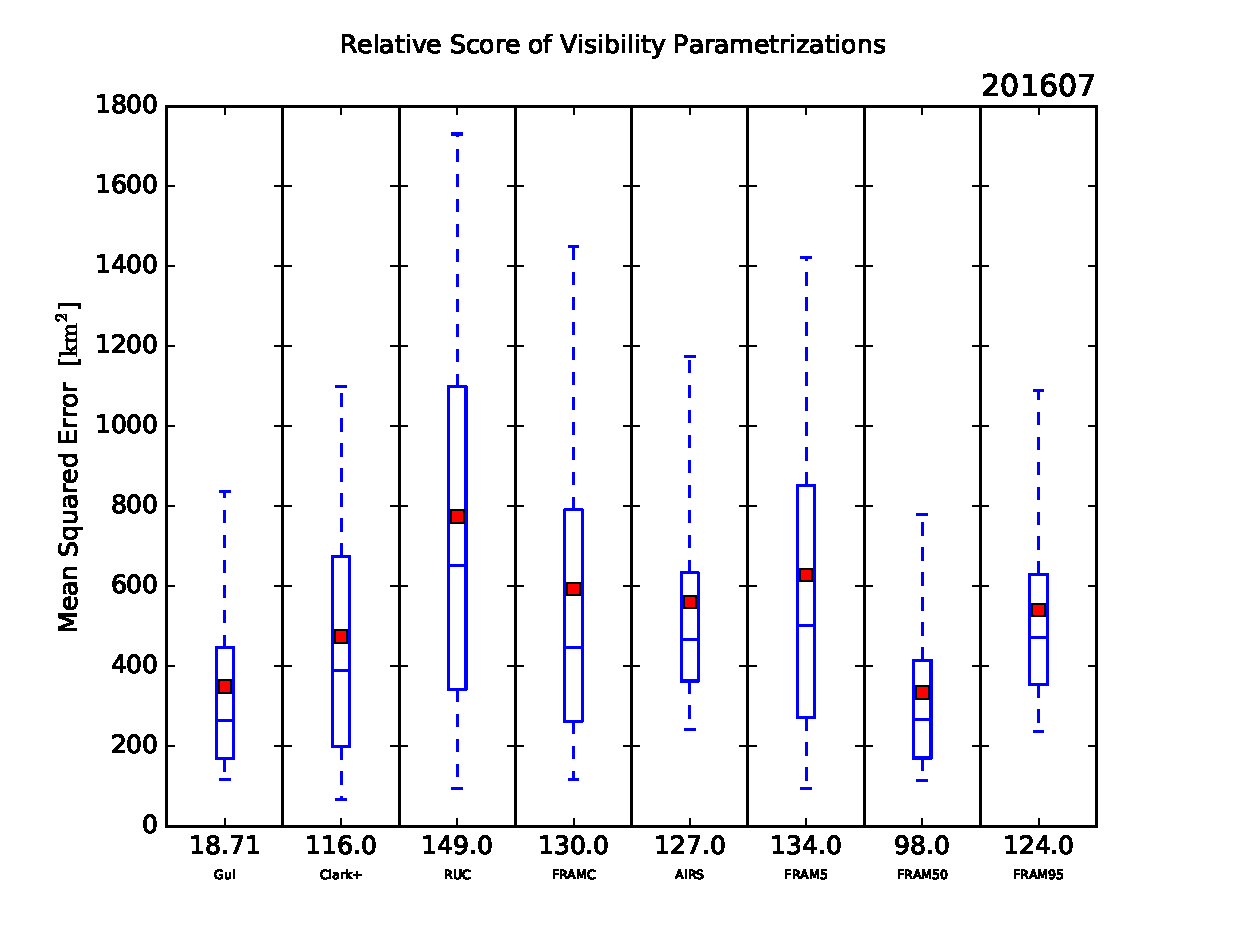
\includegraphics[width=0.8\textwidth]{graphics/results/EnsAv_RMSE_box-201607.eps}
            \caption[Box Plots of MSE, July 2016]{Box plots of the ensemble average Mean Squared Error, average for July 2016. Whiskers denoting the 5th- and the 95th-percentiles, the red squares the mean values. The first value on the X-axis is the average RMSE value of the reference parametrization `Gul' and the other values denote the Root Mean Squared Error relative to the `Gul' parametrization in percentage. }
            \label{fig:July_RMSE}
        \end{figure}

        \begin{figure}[p]
        \centering
            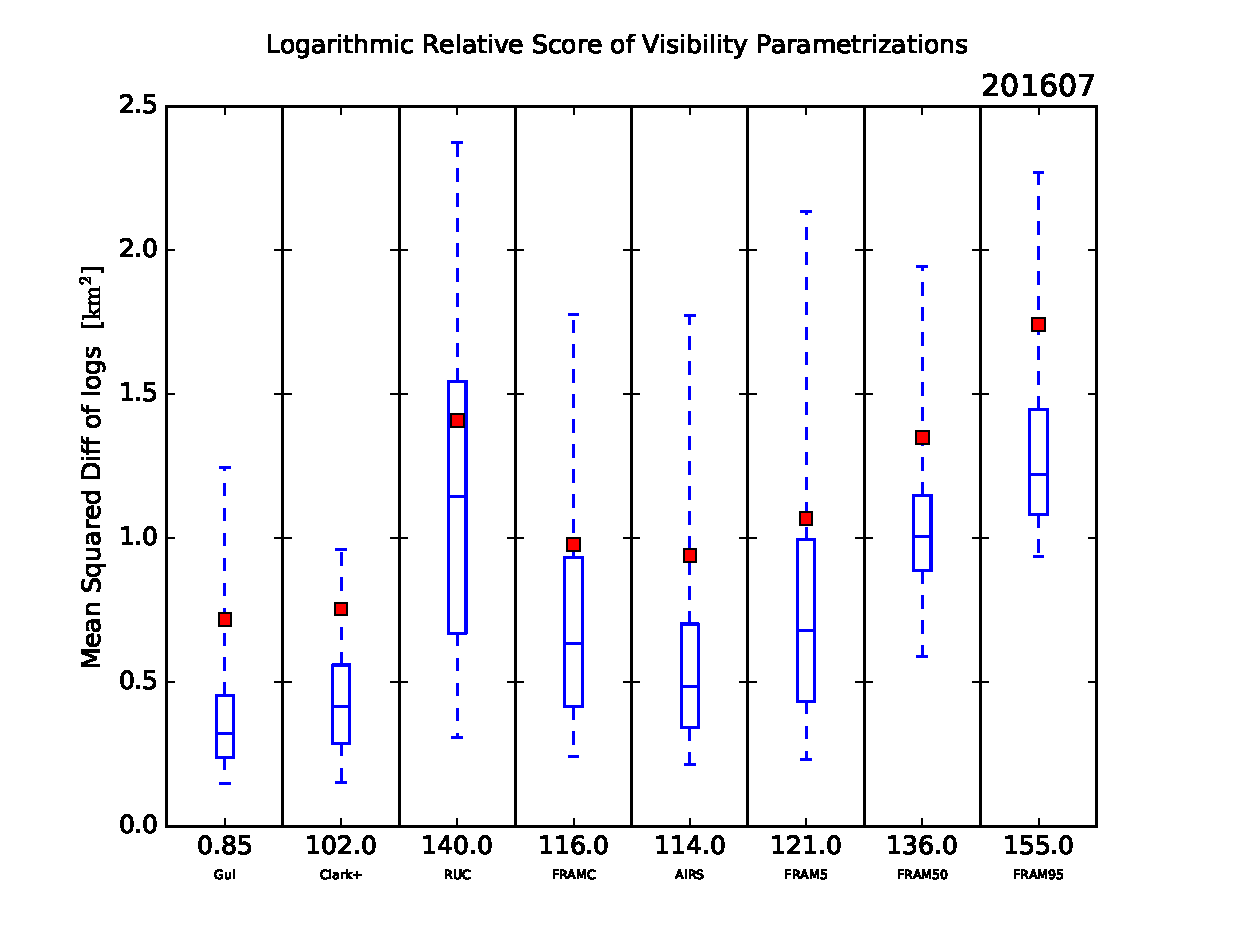
\includegraphics[width=0.8\textwidth]{graphics/results/EnsAv_logRMSE_box-201607.eps}
            \caption[Box Plots of Mean Squared Difference of Logs, July 2016]{Box plots of the ensemble average mean squared difference of the logarithmic observed and forecast values, average for July 2016. Whiskers denoting the 5th- and the 95th-percentiles, the red squares the mean values. The first value on the X-axis is the average RMSLog value of the reference parametrization `Gul' and the other values denote the RMSLog relative to the `Gul' parametrization in percentage.}
            \label{fig:July_logRMSE}
        \end{figure}
\begin{figure}[p]
    \centering
    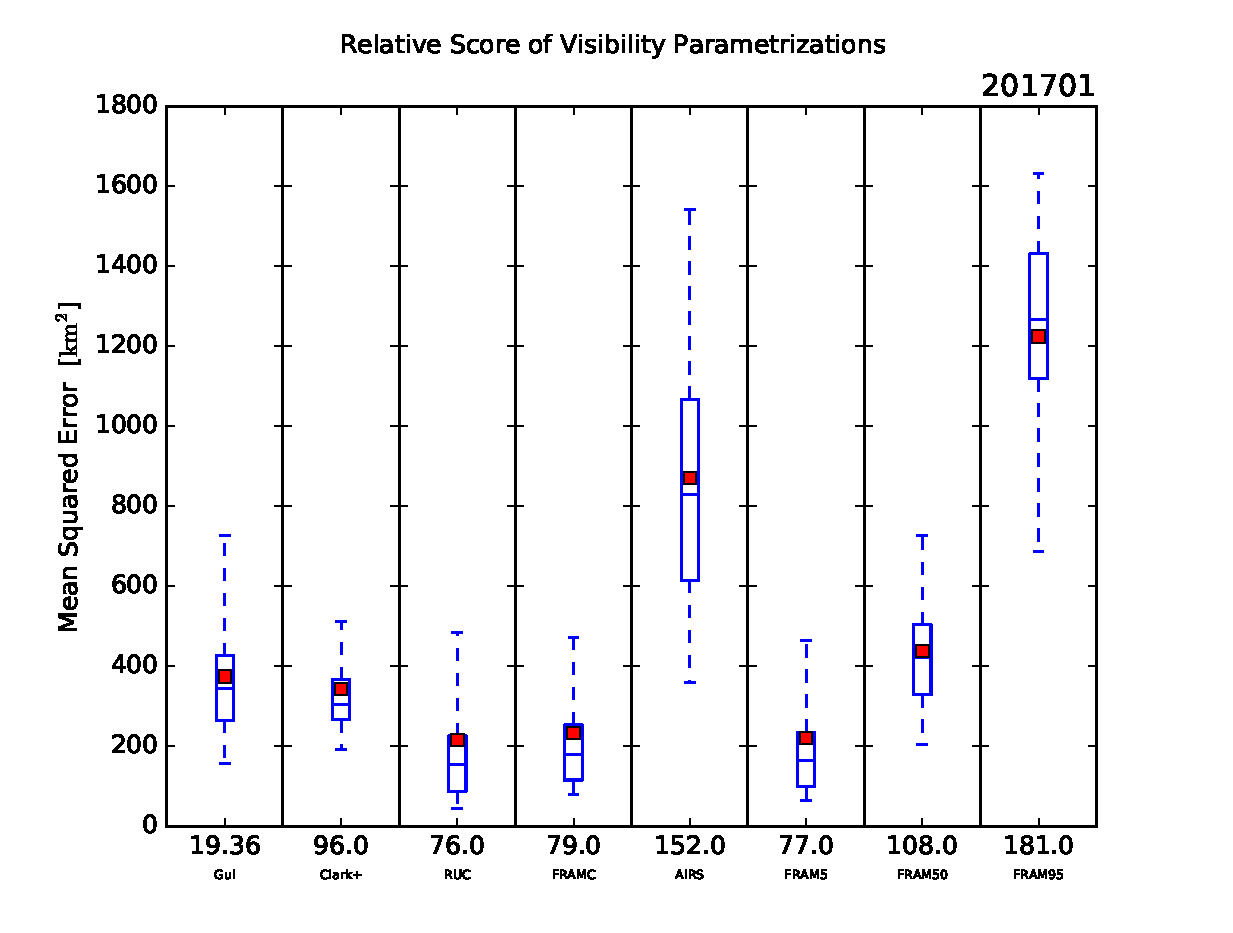
\includegraphics[width=0.8\textwidth]{graphics/results/EnsAv_RMSE_box-201701.eps}
    \caption[Box Plots of MSE, January 2017]{Box plots of the ensemble average Mean Squared Error, average for January 2017. Whiskers denoting the 5th- and the 95th-percentiles, the red squares the mean values. The first value on the X-axis is the average RMSE value of the reference parametrization `Gul' and the other values denote the  Root Mean Squared Error relative to the `Gul' parametrization in percentage.}
    \label{fig:January_RMSE}
\end{figure}
\begin{figure}[p]
    \centering
    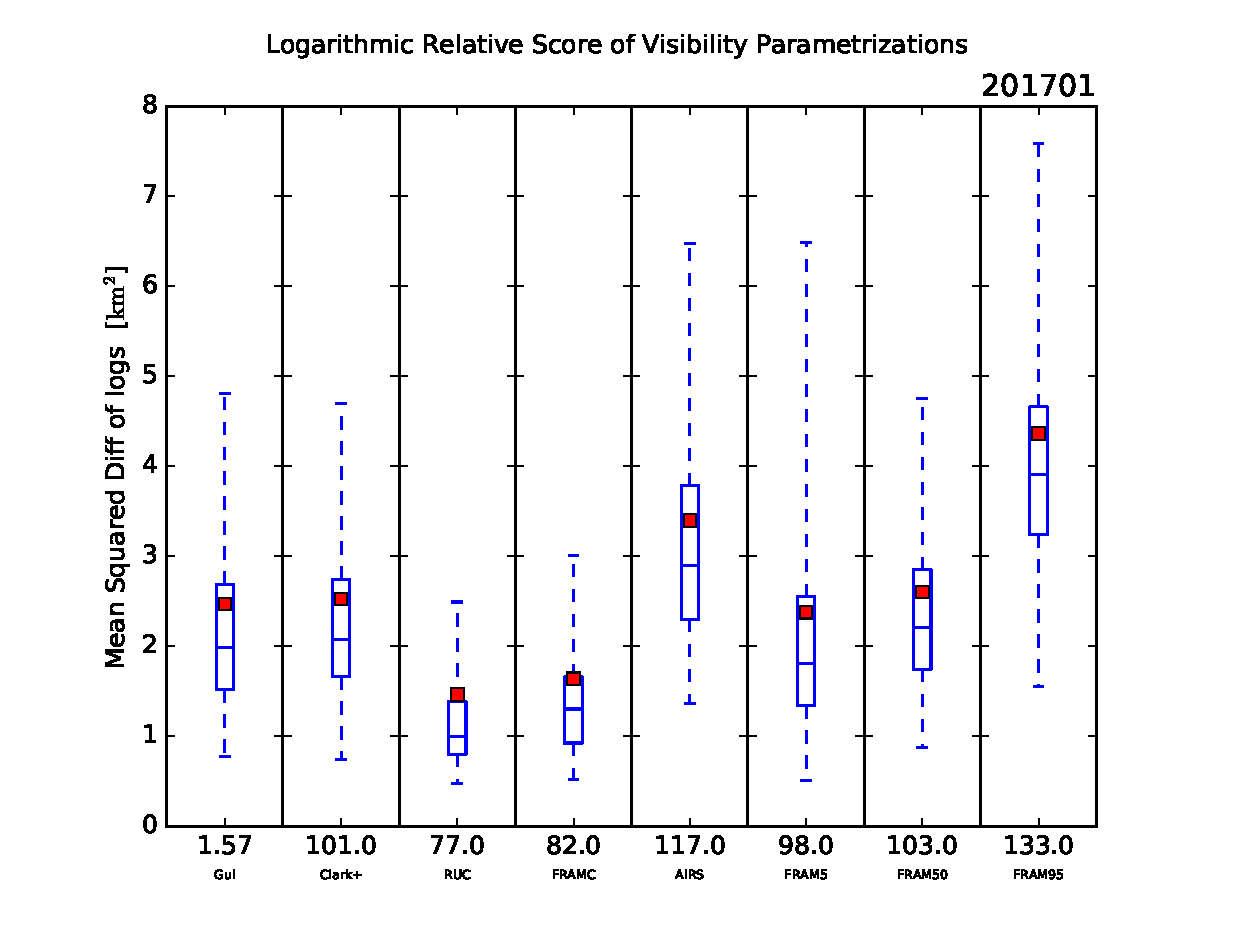
\includegraphics[width=0.8\textwidth]{graphics/results/EnsAv_logRMSE_box-201701.eps}
    \caption[Box Plots of Mean Squared Difference of Logs, January 2017]{Box plots of the ensemble average mean squared difference of the logarithmic observed and forecast values, average for January 2017. Whiskers denoting the 5th- and the 95th-percentiles, the red squares the mean values. The first value on the X-axis is the average RMSLog value of the reference parametrization `Gul' and the other values denote the RMSLog relative to the `Gul' parametrization in percentage.}
    \label{fig:January_logRMSE}
\end{figure}
\FloatBarrier


\subsubsection{Correlation of Weather Conditions and Visibility Forecast}
To understand the correlation of present weather conditions and the forecast visibility, the visibility forecast of $27^{\mathrm{th}}$ January 2017, 09:00 UTC, presented in Figure \ref{fig:cont_vis}, is discussed.\\
As shown in Figure \ref{fig: RPS_jan}, it is one of the days with a comparably high RPSS in the verification period. The satellite image in Figure \ref{fig:Satfoto} is used to analyse the weather conditions. In addition to it, the surface weather analysis in Figure \ref{fig: Bodenkarte06} and \ref{fig: Bodenkarte12} in  Appendix \ref{sec:imagesappendix} provide a qualitative overview for an enhanced interpretation of the correlation of weather conditions and forecast visibility. \\
The local RPSS values of the Clark+-parametrization for $27^{\mathrm{th}}$ January 2017 are shown in Figure \ref{fig:Rated_stations_20170127}.
The good scores in the northern part of the domain are probably the result of the stable and sunny weather conditions. 
The low visibility in some areas like the Austrian-Czech-border is due to fog. In the satellite image (Figure \ref{fig:Satfoto}) fog can be identified as the very homogeneous grey areas. Fog is forecast as liquid cloud water in the model, generally hard to predict and extremely sensitive to initial conditions \cite{zhou2012forecast}. The analysis of the results of days with a particularly good or poor performance revealed a strong correlation between the skill of the  Clark+-visibility-forecast and the skill of the forecast of liquid cloud water close to the surface. Since in this case the fog forecast had a high accuracy, the visibility forecast had a high accuracy as well. Looking at Figure \ref{fig:Satfoto}, \ref{fig: Bodenkarte06} and \ref{fig: Bodenkarte12}, we find a presence of fog in Hungary, where no reduced visibility is indicated in Figure \ref{fig:cont_vis}. The successful prediction for the northeast of Austria and the poor forecast for Hungary are reflected in the local skills illustrated in Figure \ref{fig:Rated_stations_20170127}.
\begin{figure}[h]
    \centering
    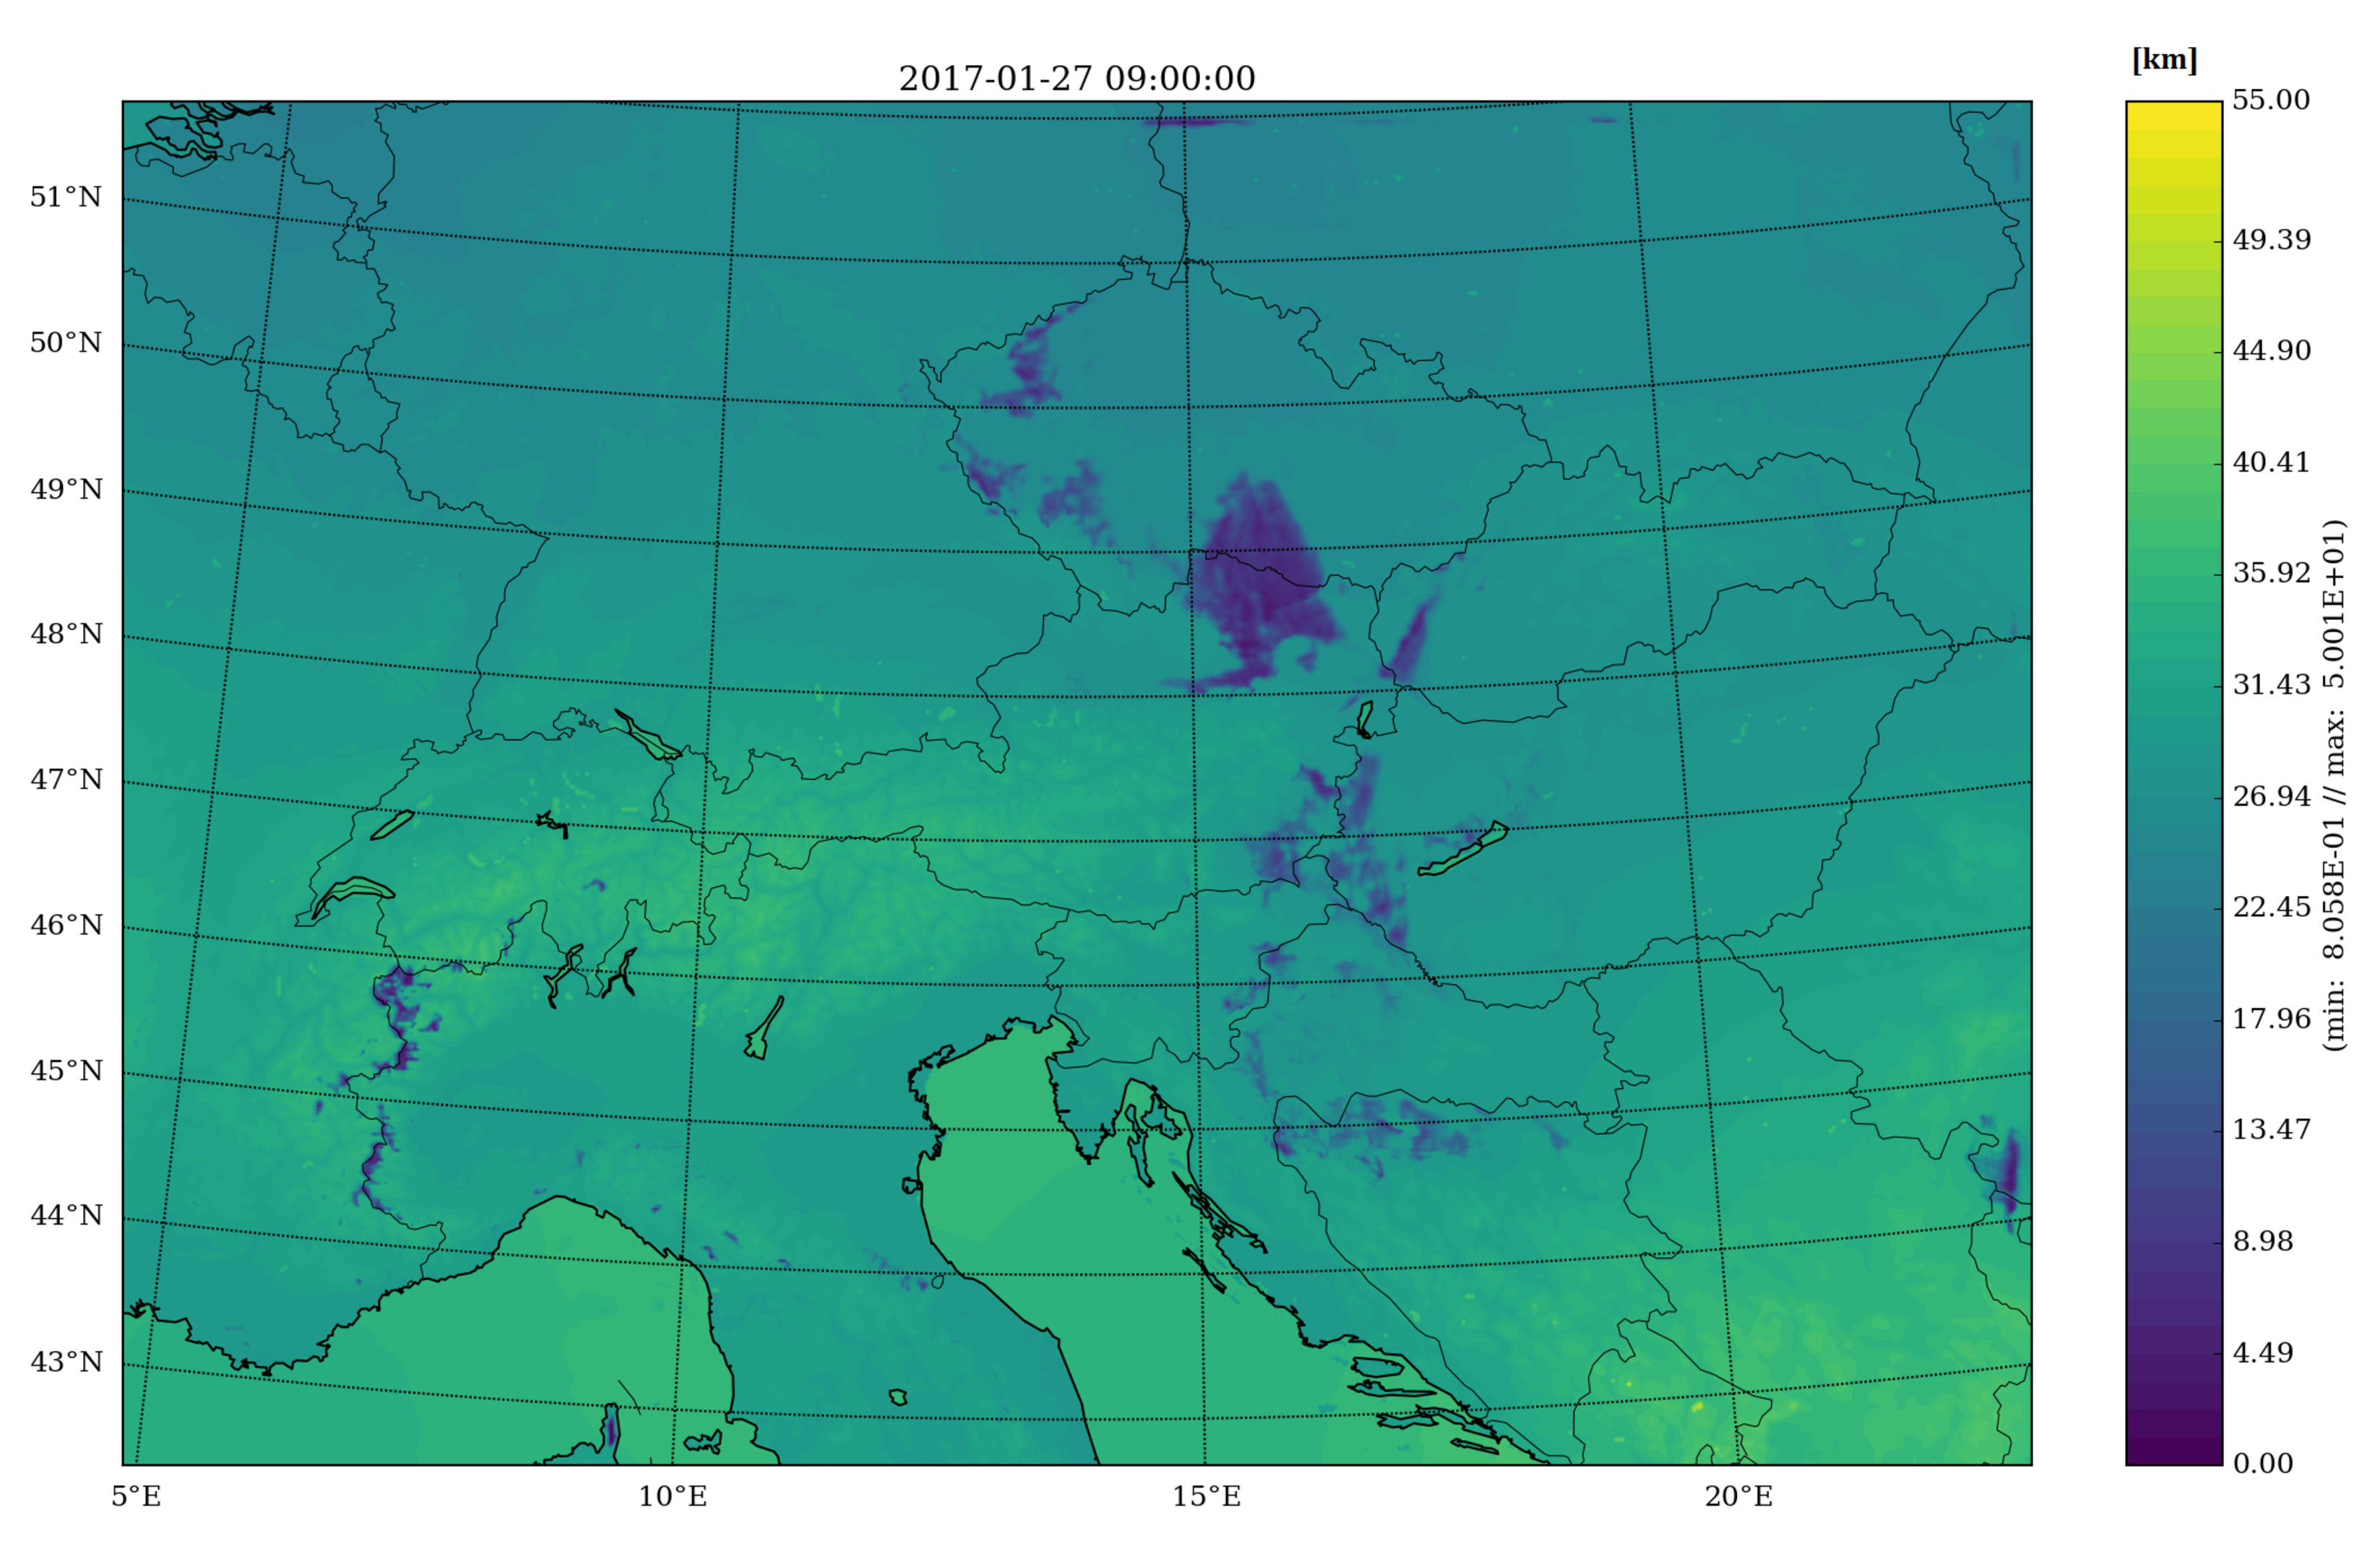
\includegraphics[width=\textwidth]{graphics/visibviri.eps}
    \caption[Contour Plot of Forecast Visibility]{Contour plot of forecast visibility by the Clark+-parametrization on 27-01-2017, 09:00 UTC. The forecast is taken from the control run from the control ensemble. }
    \label{fig:cont_vis}
\end{figure}

\begin{figure}[h]
    \centering
    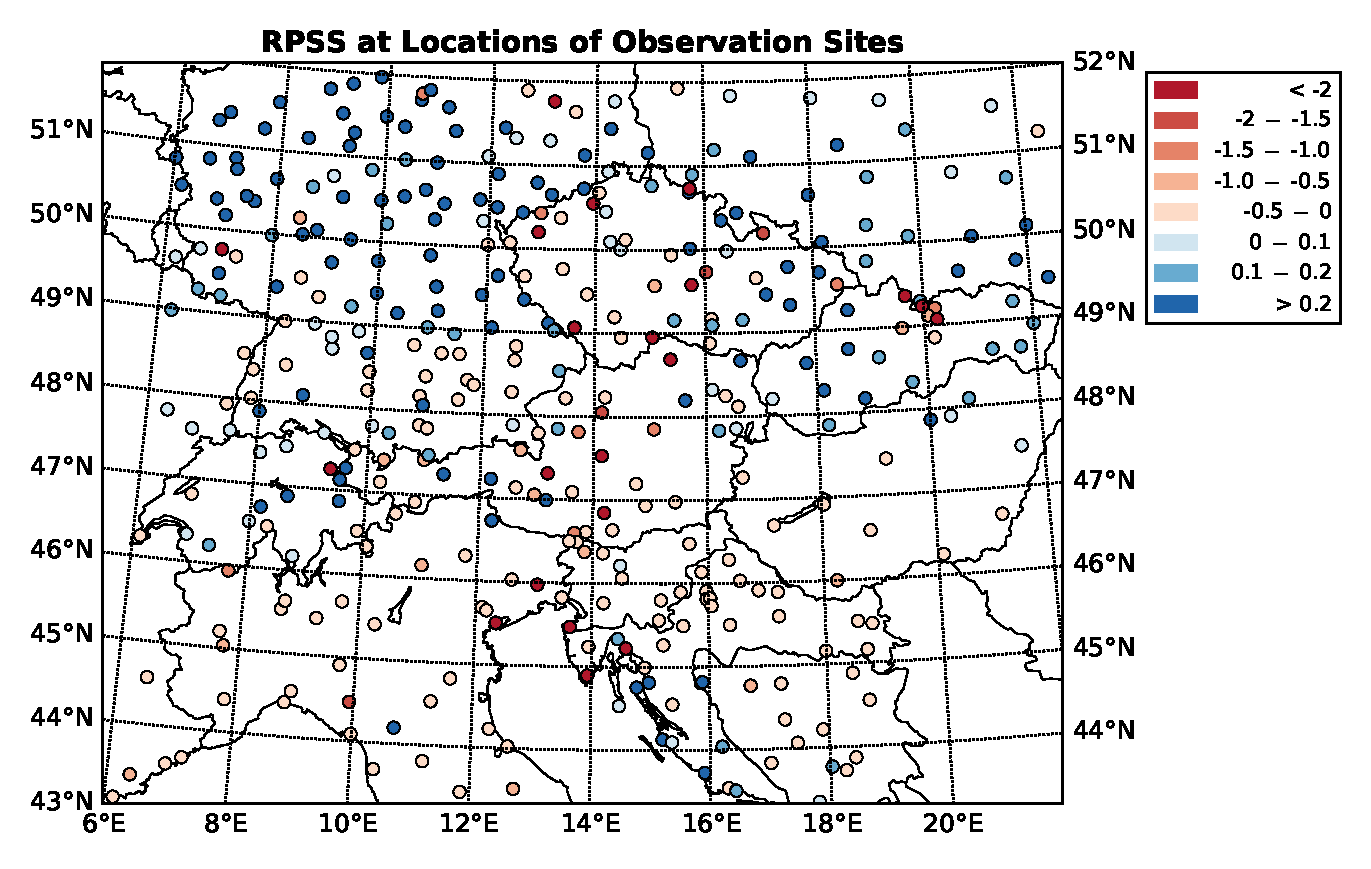
\includegraphics[width=\textwidth]{graphics/results/Rated_stations20170127.eps}
    \caption[Stations Marked with RPSS 27-01-2017]{RPSS of the Clark+-parametrization marked and colour-coded on the considered observation sites on the Austrian AROME  domain on 27-01-2017}
    \label{fig:Rated_stations_20170127}
\end{figure}


\begin{figure}[h]
    \centering
    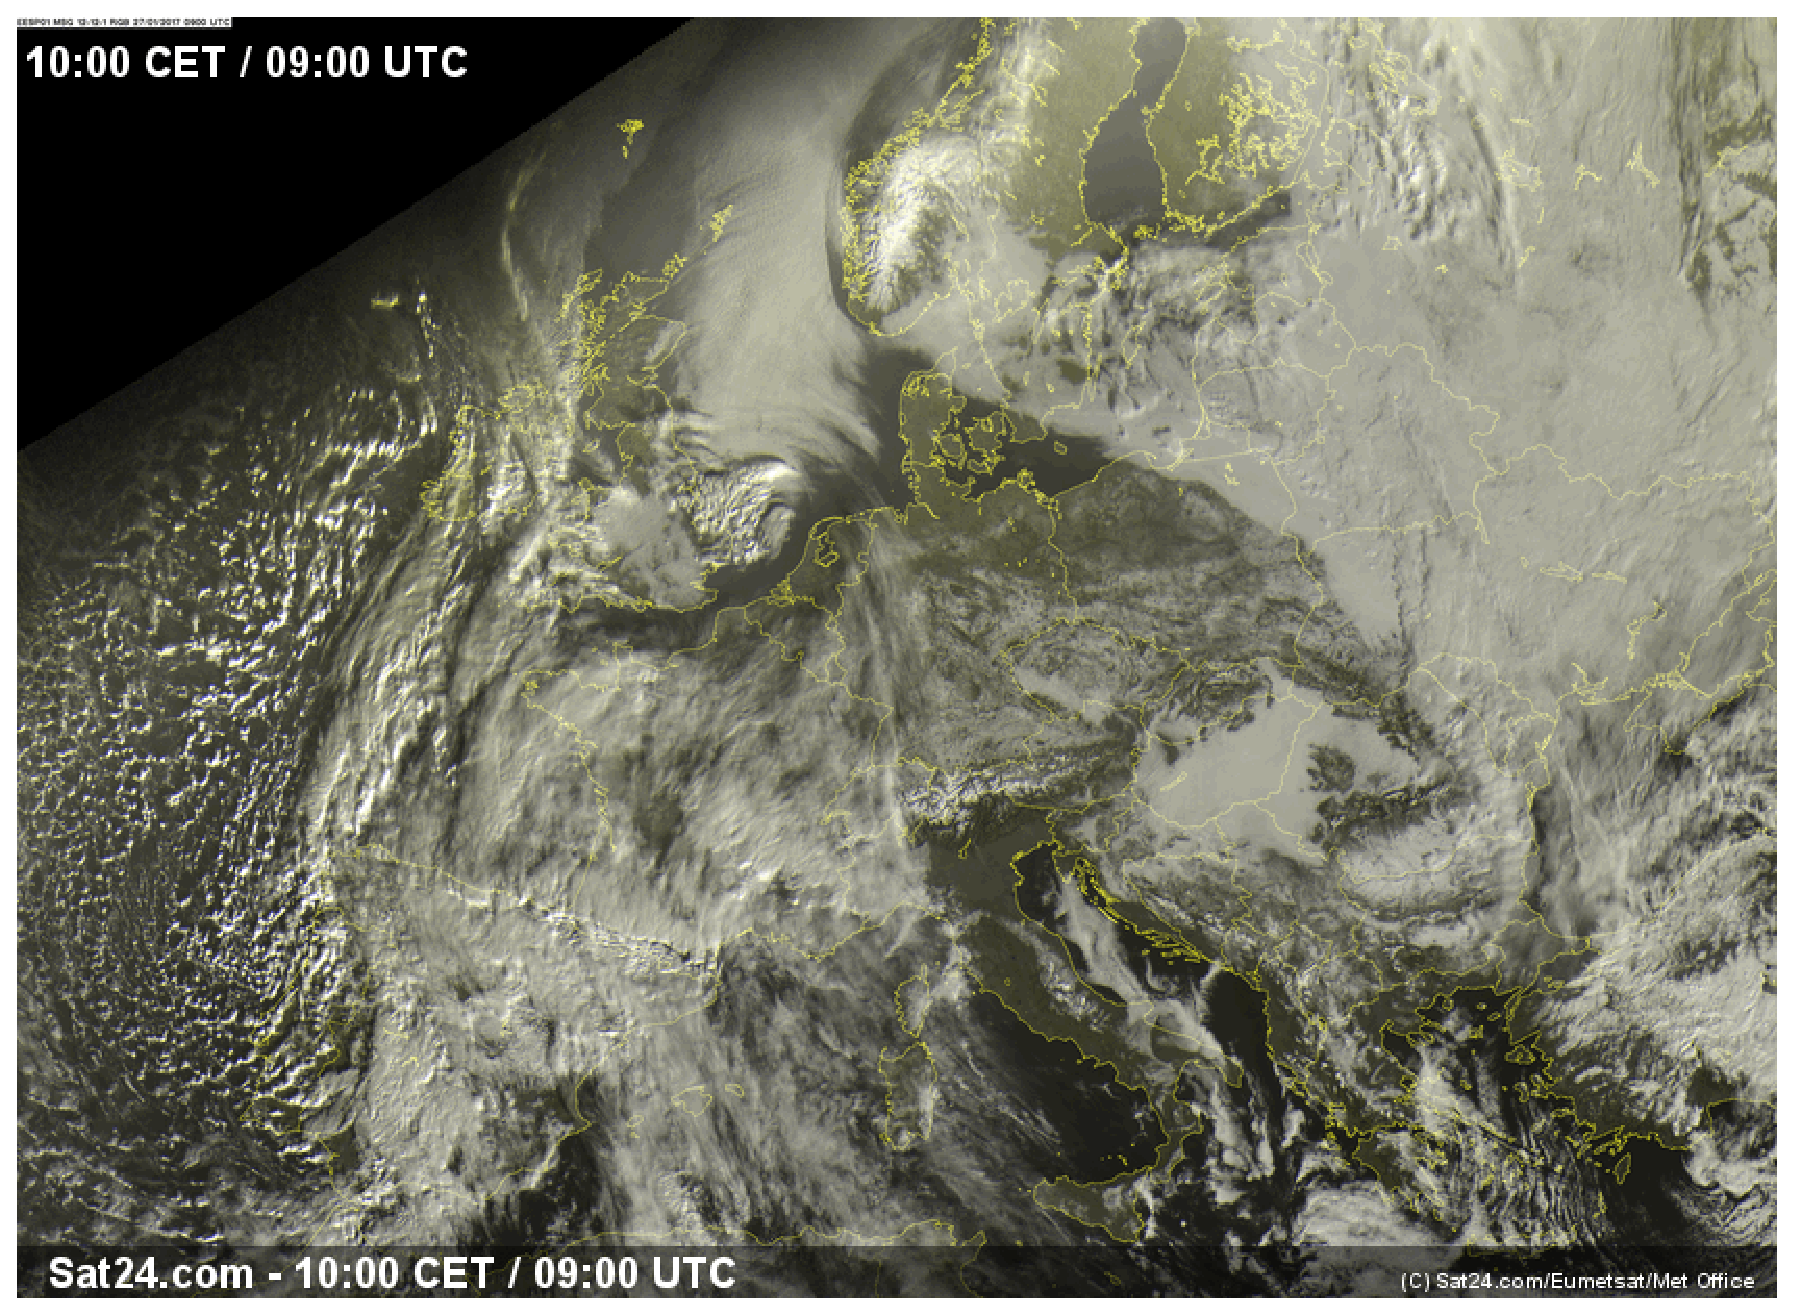
\includegraphics[width=\textwidth]{graphics/sat.eps}
    \caption[Satellite Image 27-01-2017, 09:00 UTC ]{Satellite Image 27-01-2017, 09:00 UTC 27-01-2017, 09:00 UTC of Central Europe. Image from the online archive of `\citeauthor{sat24}' \cite{sat24}}
    \label{fig:Satfoto}
\end{figure}

\FloatBarrier
\subsubsection{Seasonal Variations in Skill}
When comparing Figure \ref{fig: RPS_jan} and Figure \ref{fig: RPS_july} we see a significant difference in skill: The overall RPSS of the Clark+-parametrization is much better in January, whereas the Gul-parametrization seems to be unimpaired by seasonal changes (Figure \ref{fig:July_RMSE}, \ref{fig:July_logRMSE}, \ref{fig:January_RMSE}, \ref{fig:January_logRMSE}). This can be explained by the greater impact of the hydrometeors rain, snow, liquid cloud water and cloud ice in the Clark+-parametrization. In winter, the formation of fog is more likely due to the low saturation humidity.  Moreover, the forecast of precipitation, another parameter that impairs visibility, is more skilful in winter \cite{kidd2012}. This is suspected to be also the cause for the different effects of the perturbations observed in the case studies (Figure \ref{fig:casestudies}). Furthermore, the case studies give reason to believe that if the perturbation scheme is adapted, an increase of the RPSS of about 0.1 in January can be expected. Regarding Figure \ref{fig: RPS_jan}, it can be seen that this would result in the Clark+-parametrization outperforming the Gul-parametrization for most days in winter.\\ 
In summer, on the other hand, the clouds form higher in the atmosphere and the concentration of liquid cloud water is decreased correspondingly. In the lower levels, from which we take the input variables for the visibility module, almost no hydrometeors are present, except for rain in some cases. Although there is a dependency on the relative humidity in the Clark+-parametrization, humidity impacts the visibility only by hygroscopic growth of aerosols. But since climatological aerosol data is used, large discrepancies between the aerosol distributions in the model and the currently present aerosol distributions in the atmosphere can arise. Especially near the coast, the concentration of sea salt can vary strongly in time. Organic matter and sulphates are also effected by hygroscopic growth, but their concentrations are more stable in space and time. 
\begin{landscape}
    \begin{figure}[p]
        \centering
        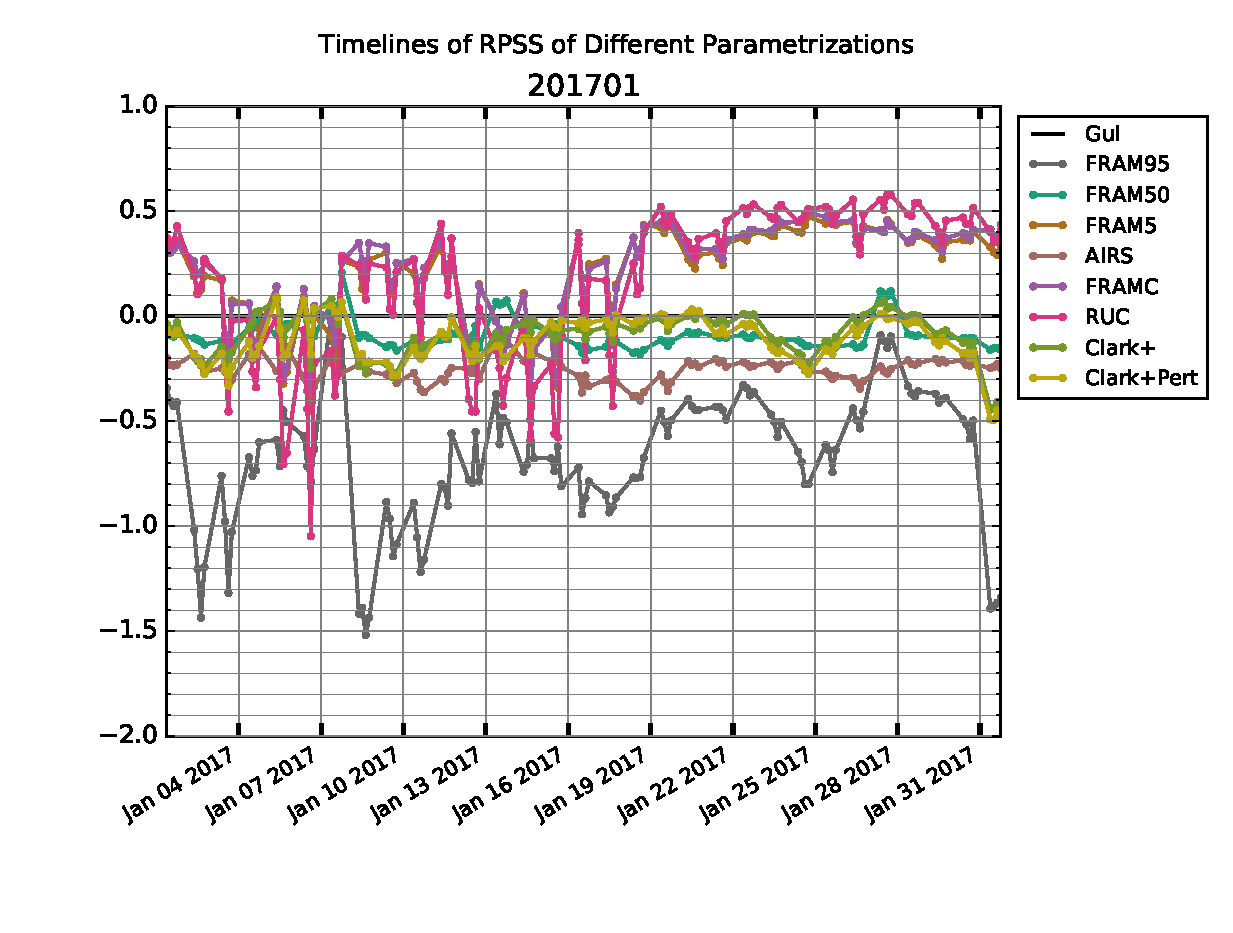
\includegraphics{graphics/results/RPS-201701.eps}
        \caption[Timeline of RPSS for January 2017 ]{RPSS versus time for January 2017. The RPSS of all parametrizations is shown: the unperturbed `Clark+', the totally perturbed `Clark+Pert' and the seven benchmark parametrizations. The black line, always 0, stands for the `Gul'-parametrization, which is the corresponding reference of the RPSS.  }
        \label{fig: RPS_jan}
    \end{figure}
    \begin{figure}[p]
        \centering
        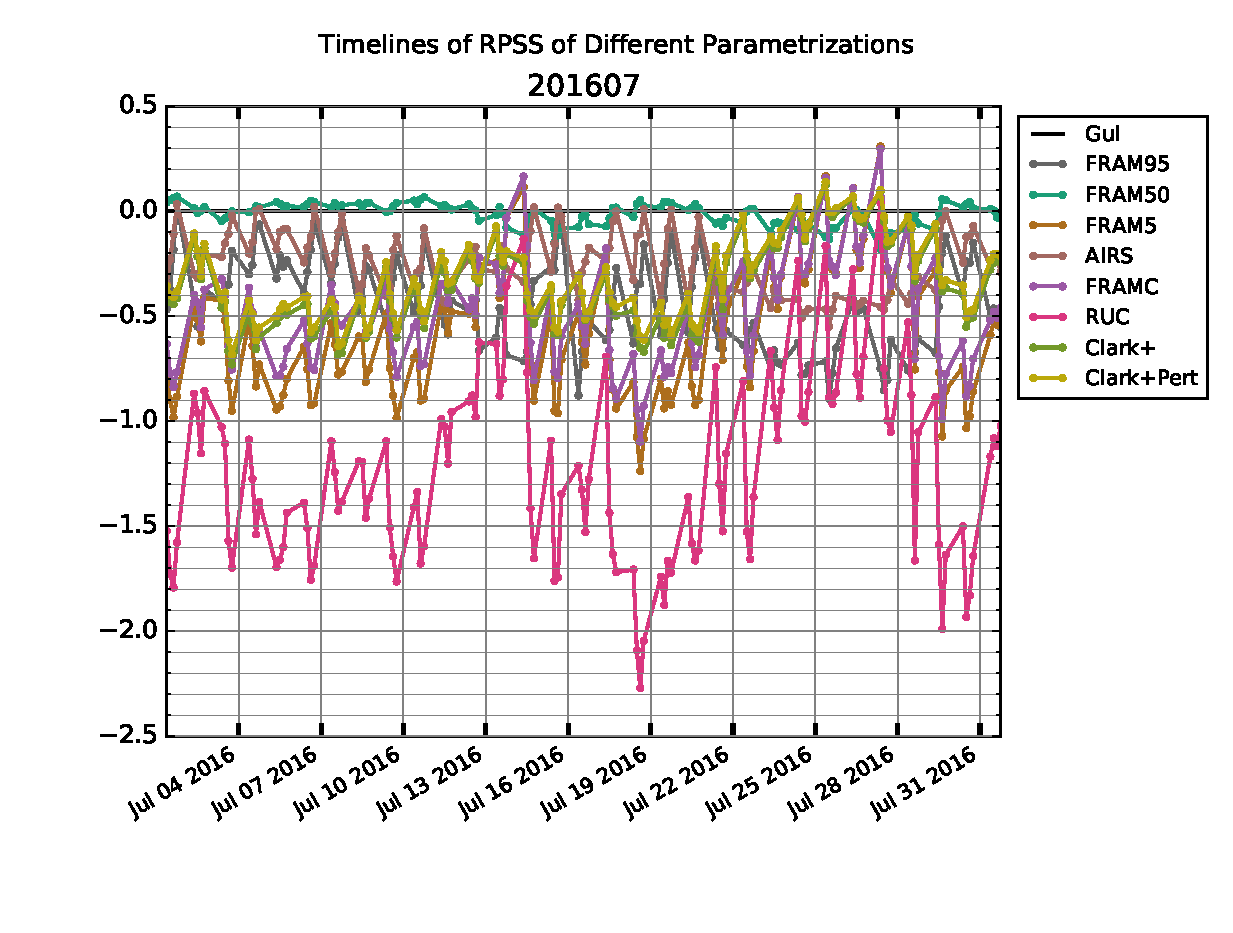
\includegraphics{graphics/results/RPS-201607.eps}
        \caption[Timeline of RPSS for July 2017]{RPSS versus time for July 2016. The RPSS of all parametrizations is shown: the unperturbed `Clark+', the totally perturbed `Clark+Pert' and the seven benchmark parametrizations. The black line, always 0, stands for the `Gul'-parametrization, which is the corresponding reference of the RPSS.}
        \label{fig: RPS_july}
    \end{figure}
\end{landscape}
\FloatBarrier

\subsubsection{Geographical Bias on the Forecast Performance }
When looking at Figure \ref{fig: RPS_jan} and \ref{fig: RPS_july}, it is evident that for some locations the chances of a skilful forecast are higher than for others. Especially along the Adriatic coast, the Clark+-parametrization performs poorly regarding to its RPSS. This is probably, because the Gul-parametrization has a direct dependence on relative humidity, which is a key parameter close to the sea. As mentioned in the discussion of the seasonal bias, sea salt concentration strongly varies, what mainly affects coastal areas. While this is the case along the coast it is noteworthy that locations in landlocked countries like in Austria or the Czech republic profit of the more complex Clark+-parametrization.

\begin{figure}[h]
    \centering
    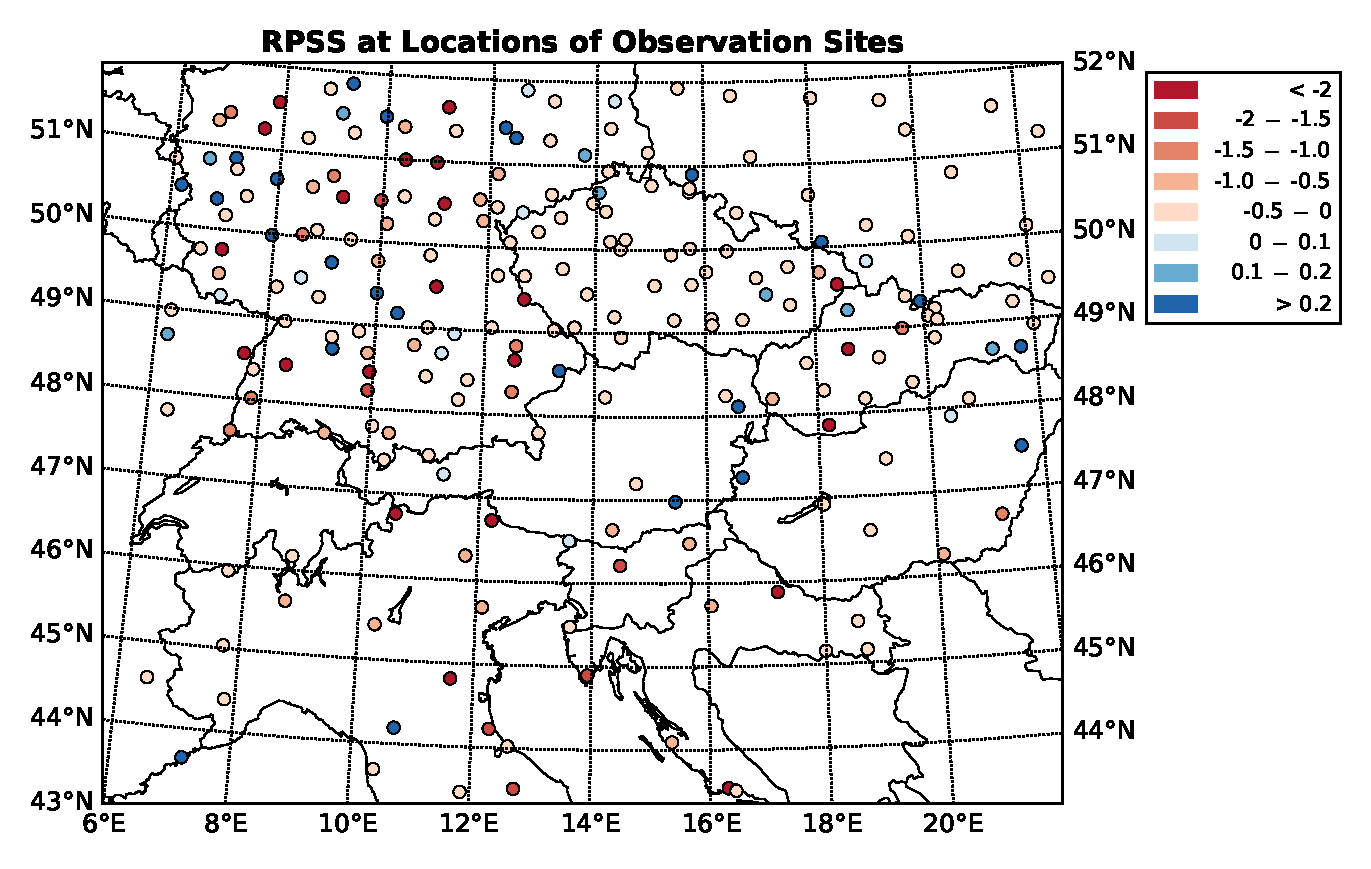
\includegraphics[width=\textwidth]{graphics/results/Rated_stations-201607.eps}
    \caption[Stations Marked with RPSS for July 2017]{RPSS of the Clark+-parametrization marked and colour-coded by value on the considered observation sites on the Austrian AROME domain for July 2016. Only observations sites for which three flawless measurements per day were available were taken into account, and are therefore shown on this plot.}
    \label{fig: Stations_july}
\end{figure}

\begin{figure}[h]
    \centering
    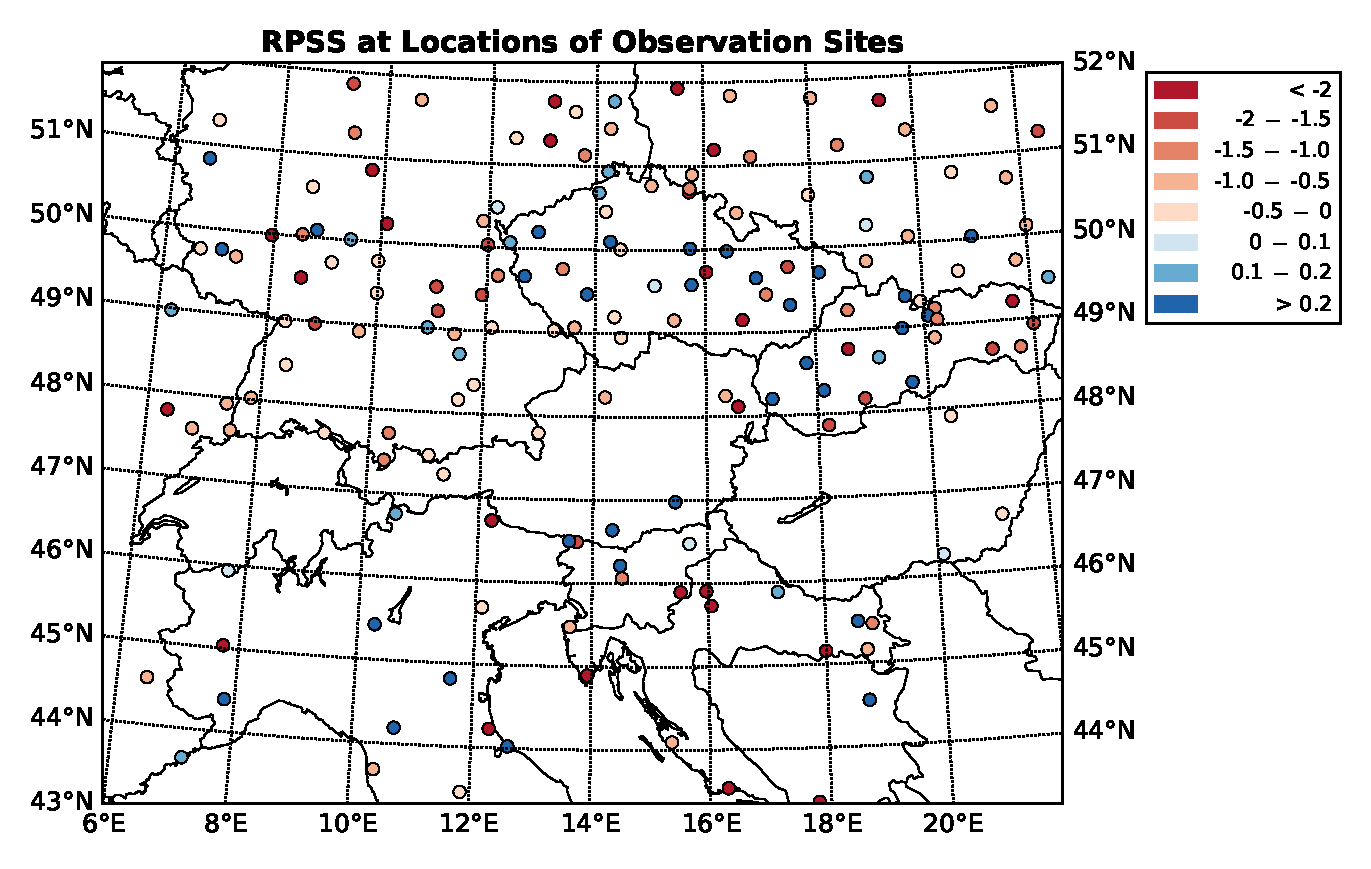
\includegraphics[width=\textwidth]{graphics/results/Rated_stations-201701.eps}
    \caption[Stations Marked with RPSS for January 2017]{RPSS of the Clark+-parametrization marked and colour-coded by value on the considered observation sites on the Austrian AROME domain for January 2017. Only observations sites for which three flawless measurements per day were available were taken into account, and are therefore marked. }
    \label{fig: Stations_jan}
\end{figure}
%\FloatBarrier

\subsubsection{Evaluation of the Perturbation Scheme}
The impact of the different variables can be investigated by analysis of the graphs in Figure \ref{fig:casestudies}. It shows the different RPSS results of the Clark+-parametrization, for the case studies, where different variables and parameters were perturbed, and also the control ensemble, where no additional perturbation was applied. Especially for the test cases in January, significant improvements can be achieved by using a suitable perturbation. But when analysing the data, we find that in some cases the added perturbation can result in a worse skill, than the one of the control ensemble. The exclusive perturbation of the aerosol concentrations `AerPert' is clearly superior to all others on the two days in winter. This was probably induced by very stable weather conditions that led to a better than average predictability of the model. Then, the uncertainties of forecast specific humidity and hydrometeor concentrations go down, but for climatological aerosol data and most constant parameters they remains the same. Figure \ref{fig:casestudies} also reveals that in winter the perturbation of the hydrometeors seems to have a bad effect on the ensemble skill, whereas in summer, it causes the ensemble skill to improve. This is due to the fact that the uncertainty of the forecast concentration of hydrometeors undergoes seasonal variations, because of the different scale of precipitation and cloud formation in winter and summer. In summer small-scale convective processes are much more influential to hydrometeor distributions than in winter  \cite{kidd2012}. \\
Future studies will likely benefit from further development of the local perturbation scheme by adjusting the amplitude of the perturbation to the present situation differently. For this study monthly climatological extrema were used to set the perturbation amplitude for each month, but the seasonally differing dynamics of precipitation, like its scale and velocities, were neglected. The major difficulty for incorporating them lies within the determination of the adjustment factor, which would require further investigation to be set properly.\\
Regarding the test cases in July, on the other hand, the totally perturbed ensemble, `TotPert', outperforms all others on average. We suspect that this behaviour is due to a greater contribution of small-scale processes  to the overall atmospheric state in summer than in winter, so the increased uncertainties let the model profit from a perturbation \cite{kidd2012}. When comparing the different single perturbations with the total perturbation, the total perturbation seems well balanced, although the perturbation of hydrometeors has clearly the strongest effect, since we can observe a significant correlation between the two ensembles.\\
The perturbation of the specific humidity always decreased the skill, except for two measurements in July, where it had no measurable effect. This is thought to be the result of an overestimation of uncertainty for the specific humidity. The specific humidity seems to be already forecast quite well by the model, which also leads to the good skill of the Gul-parametrization. \\ \\
Furthermore, the results presented in Figure \ref{fig:casestudies} show, that even a locally applied perturbation scheme can lead to more skilful ensemble forecasts and can be an alternative in cases, where a global perturbation scheme cannot be implemented. Although this was only tested for the visibility parametrization, there is no obvious reason why this should not be generalized for different parametrizations and model components.
\begin{figure}[h]
    \centering
    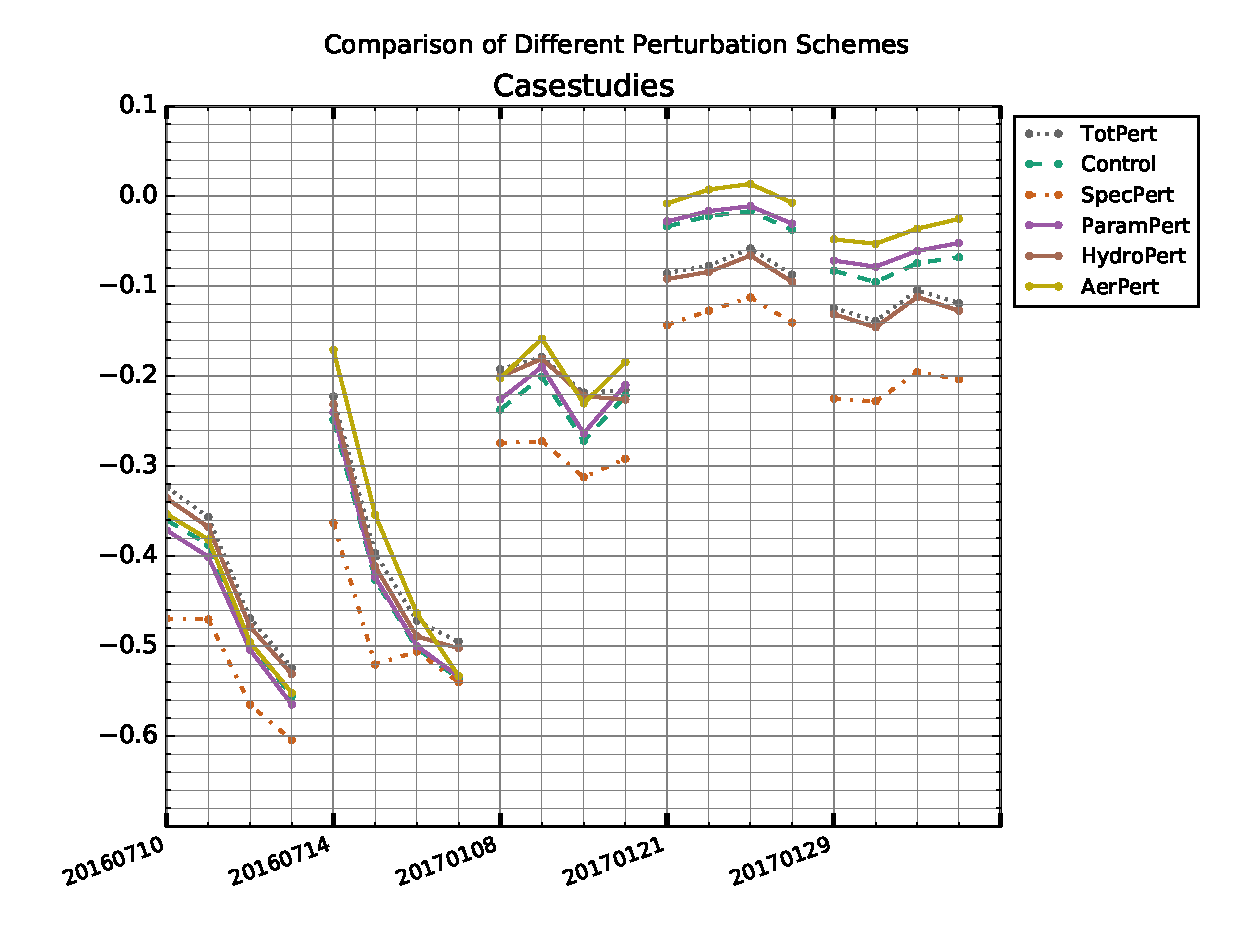
\includegraphics[width=\textwidth]{graphics/results/RPS-Casestudies.eps}
    \caption[Case studies of Different Perturbation Schemes]{RPSS  of the Clark+-parametrization for five dates in July 2016 and January 2017: the label positions of the on the x-axes indicates the skill score corresponding to the 09:00 UTC measurements and the other three following up  to 12:00, 15:00 and 18:00 UTC. The x-axes is linear for each day, but the time-frame where no measurements are taken is cut out. }
    \label{fig:casestudies}
\end{figure}
\FloatBarrier

